\documentclass[hyperref=unicode,graphics=pdflatex,13pt,xcolor={usenames,dvipsnames}]{beamer}


\usepackage[usenames,dvipsnames]{xcolor}
\usepackage[noend]{algorithmic}
\usepackage{algorithm}
\usepackage{xspace}
\usepackage[algo2e,ruled,vlined,linesnumbered]{algorithm2e}
\let\oldnl\nl% Store \nl in \oldnl
\newcommand{\nonl}{\renewcommand{\nl}{\let\nl\oldnl}}% Remove line number for one line

\usepackage{amsmath}
\usepackage{mathtools}
\usepackage{cite}
\usepackage{array}
\usepackage{multirow}
\usepackage{tabularx}
\usepackage{wasysym} %smiles

\usepackage{pgfplots}
\usepgfplotslibrary{statistics}
\usetikzlibrary{decorations.pathreplacing,calc,tikzmark}




\mode<presentation>
{
  % \usetheme{Goettingen}
%  \usecolortheme{crane}
  \setbeamercovered{invisible}
%  \useoutertheme{infolines}
%  \setbeamertemplate{headline}{} % removes the headline that infolines inserts
}

\graphicspath{{../pic/},{pic/}}

\setbeamertemplate{frametitle continuation}{(\insertcontinuationcount)}
\setbeamertemplate{footline}[text line]
{
  % \leavevmode%
  \hbox{%
    % \hspace{3mm}
    \begin{beamercolorbox}[ht=2.25ex,dp=1ex,left,wd=0.18\textwidth]{author in head/foot}%
        \usebeamerfont{author in head/foot}
        \insertshortauthor
    \end{beamercolorbox}%    
    \begin{beamercolorbox}[ht=2.25ex,dp=1ex,left,wd=0.63\textwidth]{title in head/foot}%
        \usebeamerfont{title in head/foot}
        \insertshorttitle
    \end{beamercolorbox}%
    \begin{beamercolorbox}[ht=2.25ex,dp=1ex,right,wd=0.2\textwidth]{framenumber}%
        \insertframenumber{}
        \hspace*{2ex} 
    \end{beamercolorbox}
  }%
}
\setbeamertemplate{navigation symbols}{}
\setbeamertemplate{itemize/enumerate body begin}{\normalsize}
\setbeamertemplate{itemize/enumerate subbody begin}{\normalsize}
\setbeamersize{text margin left=5mm,text margin right=5mm} 
% \setbeamerfont{page number in head/foot}{size=\large}
% \beamertemplatenavigationsymbolsempty

\usepackage[utf8]{inputenc}
\usepackage[T2A]{fontenc}
\usepackage[russian]{babel}
\usepackage{colortbl}
\usepackage{multirow}

\usepackage{algorithm}
\usepackage{algorithmic}

\newcommand\hl[1]{{\color{blue}{#1}}}
\newcommand\red[1]{{\color{red}{#1}}}
\newcommand\green[1]{{\color{green!50!darkgray}{#1}}}
\newcommand\pitem{\pause\item}

\newcommand\N{\mathbb{N}}

\deftranslation[to=russian]{Theorem}{Теорема}

\title[Вероятностные модели, условные вероятности и независимость]{Вероятностные модели, условные вероятности и независимость}

\author[Антипов Д. С.]
{Антипов Денис Сергеевич}
\institute{
Университет ИТМО, Санкт-Петербург, Россия\\
~\\
}
\date[]{
\includegraphics[height=2cm]{itmo-white-rus.png} \\
11 февраля 2022 г.}


\begin{document}

\begin{frame}[noframenumbering,plain]
%   \advance\textwidth2cm
% \hsize\textwidth
% \columnwidth\textwidth
  \titlepage
\end{frame}

\section{Введение}
\begin{frame}
  \frametitle{О лекторе}
  \begin{itemize}
    \item PhD in computer science (Университет ИТМО и {\'E}cole Polytechnique)
    \item Занимаюсь теорией \hl{эволюционных вычислений}
    \item Раньше вел матан, курс по теорверу --- второй раз
    \item Контакты:
    \begin{itemize}
      \item telegram: \href{https://t.me/antipovden}{\hl{\texttt{\underline{@antipovden}}}}
      \item email: \href{mailto:antipovden@yandex.ru}{\hl{\texttt{\underline{antipovden@yandex.ru}}}}
    \end{itemize}
    \item Обращаться ко мне на ``ты'', по имени (напомню: Денис)
    \item \hl{Не бояться} перебивать меня и задавать вопросы 
  \end{itemize}
\end{frame}

\begin{frame}
  \frametitle{О курсе}
  \begin{itemize}
    \item За основу взят \href{https://ocw.mit.edu/resources/res-6-012-introduction-to-probability-spring-2018/index.htm}{\hl{\underline{курс MIT}}}
    \item Во многом схож с курсом, который преподавала раньше Ирина Александровна Суслина
    \item Немного повторяет то, что вы проходили на дискретке
    \begin{itemize}
      \item \red{Осторожно!} Можно случайно не заметить, когда началось что-то совсем для вас новое
    \end{itemize} 
  \end{itemize}
\end{frame}

\begin{frame}
  \frametitle{Что вы уже знаете}
  \begin{itemize}
    \item Множества, операции с ними, законы де Моргана
    \item Последовательности: пределы, сходимость
    \item Ряды, порядок суммирования, сумма геометрического ряда
    \item Счетность и несчетность; почему континуум несчетен
    \item Мера и ее свойства
    \item Как интегрировать
  \end{itemize}
\end{frame}

\begin{frame}
  \frametitle{План лекции}
  \begin{itemize}
    \item Определение вероятностного пространства
    \item Условная вероятность
    \item Формула полной вероятности и формула Байеса
    \item Независимость событий, условная независимость (если успеем)
  \end{itemize}
\end{frame}

\section{Вероятностное пространство}
\begin{frame}
  \frametitle{Часть I. Вероятностное пространство}

  Вероятностное пространство --- это тройка $(\Omega, \Sigma, \Pr)$
  \begin{enumerate}
    \item \hl{$\Omega$} --- множество элементарных исходов 
    \item \hl{$\Sigma$} --- $\sigma$-алгебра событий
    \item \hl{$\Pr$} --- вероятностная мера
  \end{enumerate}
\end{frame}

\begin{frame}
  \frametitle{Множество элементарных исходов $\Omega$}

  Мы рассматриваем какой-то эксперимент, у которого возможны разные исходы. Множество всех возможных исходов и есть $\Omega$.
  \begin{itemize}
    \pitem Эксперимент не может закончиться сразу двумя исходами одновременно (исходы --- \hl{взаимоисключающие})
    \pitem Эксперимент не может закончиться исходом не из $\Omega$ ($\Omega$ --- \hl{полное})
    \pitem Множество $\Omega$ не должно быть черезчур подробным ($\Omega$ --- \hl{неизбыточное})
  \end{itemize}
\end{frame}

\begin{frame}
  \frametitle{Примеры $\Omega$}

  \begin{itemize}
    \item Подбрасывание монеты
    \begin{itemize}
      \item $\Omega = \{$орел, решка$\}$
      \pitem Если вы зануда: $\Omega = \{$орел, решка, ребро$\}$
    \end{itemize} 
    % \pitem Бросание кости
    % \begin{itemize}
    %   \item $\Omega = \{1, 2, 3, 4, 5, 6\}$
    % \end{itemize}
    \pitem Хоккейный матч (КХЛ, NHL)
    \begin{itemize}
      \item $\Omega = \{$В, ВО, ВБ, ПБ, ПО, П$\}$
      \item Если нас интересуют только очки одной команды, то $\Omega = \{0, 1, 2\}$
    \end{itemize}
    \pitem Время ожидания автобуса на остановке
    \begin{itemize}
      \item $\Omega = [0, +\infty)$
    \end{itemize}
  \end{itemize} 
\end{frame}

\begin{frame}
  \frametitle{$\sigma$-алгебра событий $\Sigma$}

  \hl{Событие} --- любое подмножество $\Omega$ ($\Leftrightarrow$ множество исходов)
  
  \pause
  \vspace{1ex}

  На $\Omega$ должна быть задана $\sigma$-алгебра событий $\Sigma$, то есть множество подмножеств, такое, что
  \begin{enumerate}
    \pitem $\emptyset \in \Sigma$
    \pitem $A \in \Sigma \Rightarrow \bar{A} \in \Sigma$
    \pitem $\{A_1, \dots, A_n, \dots\} \in \Sigma \Rightarrow \bigcap\limits_{i \in \N} A_i \in \Sigma$ и $\bigcup\limits_{i \in \N} A_i \in \Sigma$
  \end{enumerate}
\end{frame}

\begin{frame}
  \frametitle{Примеры событий}
  \begin{itemize}
    \item Домашняя команда выиграла $\{$В, ВО, ВБ$\}$
    \item Монета упала орлом $\{$орел$\}$
    \item Автобус приехал в течение 5 минут $[0, 5]$ (если считаем время в минутах)
  \end{itemize}
\end{frame}

\begin{frame}
  \frametitle{Вероятность $\Pr$}

  Вероятностная \hl{мера} $\Pr$ --- это функция, заданная на $\Sigma$, со следующими свойствами
  \begin{enumerate}
    \pitem \hl{Неотрицательность:} $\Pr(A) \ge 0$ для любого события $A$
    \pitem \hl{Нормализация:} $\Pr(\Omega) = 1$
    \pitem \hl{Счетная аддитивнотсь}: $A_1, \dots, A_n, \dots$ --- последовательность попарно непересекающихся событий, тогда
    \[
      \Pr\left(\bigcup\limits_{i \in \N} A_i\right) = \sum_{i \in \N} \Pr(A_i).
    \] 
  \end{enumerate}
  \hl{NB:} В литературе встречаются обозначения $P, p, \mathbb{P}$, их можно использовать
\end{frame}

\begin{frame}
  \frametitle{Свойства $\Pr$, следующие из аксиом}
  \begin{itemize}
    \item $\Pr(A) \le 1$
    \item $\Pr(\emptyset) = 0$
    \item $\Pr(A) + \Pr(\bar A) = 1$
    \item $A \subset B \Rightarrow \Pr(A) \le \Pr(B)$
    \item $\Pr(A \cup B) = \Pr(A) + \Pr(B) - \Pr(A \cap B)$
    \item $\Pr(A \cup B) \le \Pr(A) + \Pr(B)$ --- \hl{Union bound}
  \end{itemize}
\end{frame}

\begin{frame}
  \frametitle{Объект теории вероятности}
  \begin{itemize}
    \item Мы будем работать с вероятностным пространством $(\Omega, \Sigma, \Pr)$:
    \begin{itemize}
      \item Описывать множество элементарных исходов и определять события
      \item Задавать вероятностную меру на этих событиях
      \item Делать какие-то выводы о построенной модели
    \end{itemize}
  \end{itemize}
\end{frame}

\begin{frame}
  \frametitle{Как воспринимать нашу деятельность}
  \begin{itemize}
    \item Теорвер --- просто \hl{раздел математики}
    \begin{itemize}
      \item На основе определенных аксиом выводим какие-то более сложные утверждения и называем их теоремами
      \pitem \hl{Теорема} Вероятность события $A$ есть $p$. 
    \end{itemize}
    \pitem Как интерпретировать вероятность?
    \begin{itemize}
      \item Вероятность = \hl{частота} события (\hl{Пример:} если много раз кидать монетку, то примерно половина результатов будет ``орел'')
      \item Вероятность = \hl{наша вера в} событие (\hl{Пример:} с вероятностью 0.125 
\includegraphics[height=1em]{ska.png} выиграет в этом году кубок Гагарина)
    \end{itemize}
  \end{itemize}
\end{frame}

\begin{frame}
  \frametitle{Взаимодействие с реальным миром}
  \begin{center}
    \begin{tikzpicture}[rounded corners]
      \node (real_world) [draw, rectangle, minimum height = 1.5cm, minimum width = 3cm, fill = blue!20] at (0, 0) {Реальный мир};
      \node (theory) [draw, rectangle, minimum height = 1.5cm, minimum width = 2cm, fill = blue!20] at (7, 0) {Теорвер};
      \node (stats) [draw, rectangle, minimum height = 1.5cm, minimum width = 2.5cm, fill = blue!20] at (3.5, -3) {Статистика}; 

      \draw [->, ultra thick] (real_world) -- (stats) node [pos = 0.5, left] {Данные};
      \draw [->, ultra thick] (stats) -- (theory) node [pos = 0.5, right] {Модели};
      \draw [->, ultra thick] (theory) -- (real_world) node [pos = 0.5, above] {Предсказания};
    \end{tikzpicture}
  \end{center}
\end{frame}

\section{Условная вероятность}
\begin{frame}
  \frametitle{Часть II. Условная вероятность}
  \begin{center}
    \begin{tikzpicture}
      \draw [fill=yellow!20] (0, 0) rectangle (7, 4);
      \node [below right] at (0, 4) {$\Omega$};

      \draw [fill=green] (1.3, 1.8) circle (0.5mm);
      \draw [fill=green] (2.2, 1.3) circle (0.5mm);
      \draw [fill=green] (2.5, 1.8) circle (0.5mm);
      \draw [fill=green] (2, 2.5) circle (0.5mm);
      \draw [fill=green] (2.3, 2.7) circle (0.5mm);
      \draw [fill=green] (4, 3) circle (0.5mm);
      \draw [fill=green] (4.2, 2.7) circle (0.5mm);
      \draw [fill=green] (6, 3.4) circle (0.5mm);
      \draw [fill=green] (6.5, 0.3) circle (0.5mm);
      \draw [fill=green] (4.3, 0.9) circle (0.5mm);
      \draw [fill=green] (5, 1.8) circle (0.5mm);
      \draw [fill=green] (3.7, 1.1) circle (0.5mm);

      \onslide<2->{
        \draw [fill=blue, fill opacity=0.2] (2, 2) ellipse (10mm and 15mm);
        \node [red] at (1.5, 3) {$A$};
      }

      \onslide<3->{
        \draw [fill=red, fill opacity=0.2] (2, 0) rectangle (7, 2);
        \node [blue, below left] at (7, 2) {$B$};
      }
    \end{tikzpicture}  
  \end{center}
  \begin{itemize}
    \item Пусть все исходы равновероятны (вероятность каждого $\tfrac{1}{12}$)
    \pitem Вероятность события $A$ есть $\Pr(A) = 5\cdot \tfrac{1}{12} = \frac{5}{12}$
    \pitem Нам стало известно, что произошло событие $B$. Какой стала вероятность события $A$?
    \pitem В событие $B$ входят 6 равновероятных исходов, из которых только 2 входят в событие $A$. То есть теперь вероятность события $A$ есть $2 \cdot \tfrac{1}{6} = \tfrac {1}{3}$. 
  \end{itemize}
\end{frame}

\begin{frame}
  \frametitle{Поступление новой информации}
  \begin{center}
    \scalebox{0.4}{
      \begin{tikzpicture}
        \draw [fill=yellow!20] (0, 0) rectangle (7, 4);
        \node [below right] at (0, 4) {$\Omega$};
  
        \draw [fill=green] (1.3, 1.8) circle (0.5mm);
        \draw [fill=green] (2.2, 1.3) circle (0.5mm);
        \draw [fill=green] (2.5, 1.8) circle (0.5mm);
        \draw [fill=green] (2, 2.5) circle (0.5mm);
        \draw [fill=green] (2.3, 2.7) circle (0.5mm);
        \draw [fill=green] (4, 3) circle (0.5mm);
        \draw [fill=green] (4.2, 2.7) circle (0.5mm);
        \draw [fill=green] (6, 3.4) circle (0.5mm);
        \draw [fill=green] (6.5, 0.3) circle (0.5mm);
        \draw [fill=green] (4.3, 0.9) circle (0.5mm);
        \draw [fill=green] (5, 1.8) circle (0.5mm);
        \draw [fill=green] (3.7, 1.1) circle (0.5mm);

        \draw [fill=blue, fill opacity=0.2] (2, 2) ellipse (10mm and 15mm);
        \node [red] at (1.5, 3) {$A$};

        \draw [fill=red, fill opacity=0.2] (2, 0) rectangle (7, 2);
        \node [blue, below left] at (7, 2) {$B$};
      \end{tikzpicture} 
    }
  \end{center}
  \begin{itemize}
    \item При появлении новой информации мы хотим изменить свою модель, чтобы она соответствовала новым \hl{условиям}
    \pitem Пусть мы знаем, что произошло событие \hl{$B$}. Тогда мы хотим:
    \begin{itemize}
      \item $A: A \cap B = \emptyset \Rightarrow \Pr(A \mid B) = 0$
      \pitem $A \subset B \Rightarrow \Pr(A \mid B) = \frac{\Pr(A)}{\Pr(B)}$ (сохраняем \hl{нормализацию}) 
    \end{itemize}
    \pitem Любое событие можно представить как $A = (A \cap B) \cup (A \cap \bar B)$, тогда по аддитивности вероятности 
    \[
      \Pr(A \mid B) = \Pr(A \cap B \mid B) + \Pr(A \cap \bar B \mid B) = \frac{\Pr(A \cap B)}{\Pr(B)} + 0.
    \]
  \end{itemize}
\end{frame}

\begin{frame}
  \frametitle{Определение условной вероятности}
  \begin{center}
      \begin{tikzpicture}[rounded corners]
        \node [draw, rectangle, fill=blue!20, minimum height = 1.5cm, minimum width = 2.5cm] at (0,0) {$\Pr(A \mid B) = \frac{\Pr(A \cap B)}{\Pr(B)}$};
      \end{tikzpicture}
  \end{center}

  \vspace{1em}

  $\Pr(A \mid B)$ --- Вероятность события $A$ \hl{при условии} события $B$

  \vspace{1em}
  \pause

  \hl{NB:} $\Pr(\cdot \mid B)$ --- это новая вероятностная мера, заданная на той же самой $\sigma$-алгебре, то есть для нее выполняются все аксиомы меры и следствия из них
\end{frame}

\begin{frame}
  \frametitle{Пример условной вероятности}
  \begin{columns}
    \begin{column}{0.5\textwidth}
    Бросок двух тетраидальных костей  
      \begin{center}
        \begin{tikzpicture}
          \onslide<2->{
            \fill [blue!50] (1, 1) rectangle (4, 4);
            \fill [white] (2, 2) rectangle (4, 4);
          }

          \onslide<3>{
            \fill [red!50] (0, 0) rectangle (1, 1);
          }
          \onslide<4>{
            \fill[red!50] (0, 3) rectangle (1,4);
            \fill[red, opacity = 0.5] (1, 2) rectangle (2,3);
            \fill[red, opacity = 0.5] (2, 1) rectangle (3,2);
            \fill[red!50] (3, 0) rectangle (4,1);
          }
          \onslide<5>{
            \fill[red, opacity = 0.5] (0, 1) rectangle (4, 2);
          }

          \draw [step=1.0] (0, 0) grid (4, 4);

          \draw [draw = none] (-0.8, 0) -- (-0.8, 4) node [pos=0.5, sloped] {Первая кость $X$};
          \node [left] at (0, 0.5) {1};
          \node [left] at (0, 1.5) {2};
          \node [left] at (0, 2.5) {3};
          \node [left] at (0, 3.5) {4};

          \node at (2, -0.8) {Вторая кость $Y$};
          \node [below] at (0.5, 0) {1};
          \node [below] at (1.5, 0) {2};
          \node [below] at (2.5, 0) {3};
          \node [below] at (3.5, 0) {4};
        \end{tikzpicture}
      \end{center}
    \end{column}
    \begin{column}{0.5\textwidth}
      \pause
      Событие \hl{$B$}: $\min\{X, Y\} = 2$
      \begin{itemize}
        \pitem $\Pr(\red{\max\{X, Y\} = 1} \mid B) = 0$ 
        \pitem $\Pr(\red{X + Y = 5} \mid B) = \frac{2}{5}$
        \pitem $\Pr(\red{X = 2} \mid B) = \frac{3}{5}$
      \end{itemize}
    \end{column}
  \end{columns}
\end{frame}

\begin{frame}
  \frametitle{Модели с условной вероятностью}
  \begin{columns}
    \begin{column}{0.6\textwidth}
      \begin{itemize}
        \item В HoMM3 у вашего героя экспертный навык удачи 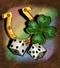
\includegraphics[height=1.5em]{luck.jpg}
        \item Ваш титан 
\includegraphics[height=2em]{titan.png} атакует дендройда 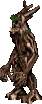
\includegraphics[height=2em]{dendroid.png} 
        \begin{itemize}
          \small
          \pitem Урон титана 40-60 (выбирается равновероятно)
          \item Здоровье дендройда 55
          \item Пусть навыки атаки и защиты одинаковы
          \item Удача срабатывает с вероятностью 0.125 и удваивает урон 
        \end{itemize}
        \pitem Событие \hl{$A$}: сработала удача
        \item Событие \red{$B$}: дендройд пал
      \end{itemize}
    \end{column}
    \begin{column}{0.4\textwidth}
      \pause
      \begin{center}
        \begin{tikzpicture}
          \node (A) at (1.5, 1.5) {\hl{$A$}};
          \node (notA) at (1.5,  -1.5) {\hl{$\bar A$}};
          \node (BA) at (3, 3) {\red{$B$}};
          \node (notBA) at (3, 1) {\red{$\bar B$}};
          \node (BnotA) at (3, -1) {\red{$B$}};
          \node (notBnotA) at (3, -3) {\red{$\bar B$}};

          \draw (0, 0) -- (A);
          \draw (0, 0) -- (notA);
          \draw (A) -- (BA);
          \draw (A) -- (notBA);
          \draw (notA) -- (BnotA);
          \draw (notA) -- (notBnotA);

          \onslide<5->{
            \node [above left] at (0.75, 0.75) {\tiny$\Pr(\hl{A}) = 0.125$};
            \node [below left] at (0.75, -0.75) {\tiny$\Pr(\hl{\bar A}) = 0.875$};
          }
          \onslide<6->{
            \node [above left] at (2.25, 2.25) {\tiny{$\Pr(\red{B} \mid \hl{A}) = 1$}};
            \node [below] at (2, 1.125) {\tiny{$\Pr(\red{\bar B} \mid \hl{A}) = 0$}};
            \node [above] at (2, -1.125) {\tiny{$\Pr(\red{B} \mid \hl{\bar A}) = 6/21$}};
            \node [below left] at (2.25, -2.25) {\tiny{$\Pr(\red{\bar B} \mid \hl{\bar A}) = 15/21$}};
          }
        \end{tikzpicture}
      \end{center}
    \end{column}
  \end{columns}
\end{frame}

\begin{frame}
  \frametitle{Модели с условной вероятностью}
  \begin{columns}
    \begin{column}{0.6\textwidth}

      \[
        \Pr(\red{B} \mid \hl{A}) = \frac{\Pr(\red{B} \cap \hl{A})}{\Pr(\hl{A})}
      \]
      
      \vspace{2em}
      \begin{itemize}
        \item $\Pr(\hl{A} \cap \red{B}) =$ \onslide<2->{$\Pr(\hl{A})\Pr(\red{B} \mid \hl{A}) = 0.125$}
        \onslide<3->{
          \item $\Pr(\red{B}) =$ 
        }
        \vspace{1em}
        \onslide<4->{
          $\Pr(\red{B} \cap \hl{A}) + \Pr(\red{B} \cap \hl{\bar A}) = \Pr(\hl{A})\Pr(\red{B} \mid \hl{A}) + \Pr(\hl{\bar A})\Pr(\red{B} \mid \hl{\bar A}) = 0.125 \cdot 1 + 0.875 \cdot \tfrac{6}{21} = 0.375$ 
        }
        \vspace{1em}
        \onslide<5->{
          \item $\Pr(\hl{A} \mid \red{B}) =$
        }
        \onslide<6->{
          $\frac{\Pr(\hl{A} \cap \red{B})}{\Pr(\red{B})}  = \frac{0.125}{0.375} = \frac{1}{3}$
        }
      \end{itemize}
    \end{column}
    \begin{column}{0.4\textwidth}
      \begin{center}
        \begin{tikzpicture}
          \node (A) at (1.5, 1.5) {\hl{$A$}};
          \node (notA) at (1.5,  -1.5) {\hl{$\bar A$}};
          \node (BA) at (3, 3) {\red{$B$}};
          \node (notBA) at (3, 1) {\red{$\bar B$}};
          \node (BnotA) at (3, -1) {\red{$B$}};
          \node (notBnotA) at (3, -3) {\red{$\bar B$}};

          \draw (0, 0) -- (A);
          \draw (0, 0) -- (notA);
          \draw (A) -- (BA);
          \draw (A) -- (notBA);
          \draw (notA) -- (BnotA);
          \draw (notA) -- (notBnotA);

          \onslide<2>{
            \draw [ultra thick, red] (0, 0) -- (A) -- (BA);
          }
          \onslide<4>{
            \draw [ultra thick, red] (0, 0) -- (A) -- (BA);
            \draw [ultra thick, red] (0, 0) -- (notA) -- (BnotA);
          }

          \node [above left] at (0.75, 0.75) {\tiny$\Pr(\hl{A}) = 0.125$};
          \node [below left] at (0.75, -0.75) {\tiny$\Pr(\hl{\bar A}) = 0.875$};

          \node [above left] at (2.25, 2.25) {\tiny{$\Pr(\red{B} \mid \hl{A}) = 1$}};
          \node [below] at (2, 1.125) {\tiny{$\Pr(\red{\bar B} \mid \hl{A}) = 0$}};
          \node [above] at (2, -1.125) {\tiny{$\Pr(\red{B} \mid \hl{\bar A}) = 6/21$}};
          \node [below left] at (2.25, -2.25) {\tiny{$\Pr(\red{\bar B} \mid \hl{\bar A}) = 15/21$}};
        \end{tikzpicture}
      \end{center}
    \end{column}
  \end{columns}
\end{frame}

\begin{frame}
  \frametitle{Правило (теорема) умножения вероятностей}

  \begin{itemize}
    \item Мы уже видели, что $\Pr(A \cap B) = \Pr(A) \Pr(B \mid A)$
    \item Можно обобщить:
    \begin{center}
      \begin{tikzpicture}[rounded corners]
        \node [draw, rectangle, fill=blue!20] at (0, 0) {\begin{minipage}{\linewidth}
          $$\Pr\left(\bigcap\limits_{i = 1}^n A_i\right) = \Pr(A_1) \prod_{i = 2}^n \Pr(A_i \mid A_1 \cap \dots \cap A_{i - 1})$$
        \end{minipage}};
      \end{tikzpicture}
    \end{center}  
    \pitem Докажем по индукции
  \end{itemize}

  \begin{align*}
    \Pr\left(\bigcap\limits_{i = 1}^n A_i\right) &= \Pr\left(A_n \cap \left(\bigcap\limits_{i = 1}^{n - 1} A_i\right)\right) \\
      \onslide<3->{&= \Pr\left(\bigcap\limits_{i = 1}^{n - 1} A_i\right) \Pr\left(A_n \mid \left(\bigcap\limits_{i = 1}^{n - 1} A_i\right)\right) \pause \\}
      \onslide<4->{&= \Pr(A_1) \prod_{i = 2}^n \Pr(A_i \mid A_1 \cap \dots \cap A_{i - 1})}
  \end{align*}
\end{frame}

\begin{frame}
  \frametitle{Правило (теорема) полной вероятности}
  \begin{columns}
    \begin{column}{0.4\textwidth}
      \begin{tikzpicture}
        \draw [fill=yellow!20] (0, 0) rectangle (4, 3);
        \node [below right] at (0, 3) {$\Omega$};

        \draw [fill=blue, fill opacity=0.3] (2, 1.5) ellipse (1.2cm and 0.75cm);
        \node at (1.5, 2) {\red{$B$}}; 

        \draw (0, 0.8) -- (2, 1.2) -- (3, 3);
        \draw (2, 1.2) -- (4, 0);
        \node [right] at (0, 2) {\hl{$A_1$}};
        \node [below left] at (4, 3) {\hl{$A_2$}};
        \node [above right] at (0, 0) {\hl{$A_3$}};
      \end{tikzpicture}
    \end{column}
    \begin{column}{0.6\textwidth}
      Есть разбиение $\Omega$ на события $\hl{A_1}, \hl{A_2}, \hl{A_3}, \dots$
      
      \begin{itemize}
        \item Знаем $\Pr(\hl{A_i})$ для всех $i$
        \item Знаем $\Pr(\red{B} \mid \hl{A_i})$ для всех $i$
      \end{itemize}

      \pause

      \begin{center}
        \begin{tikzpicture}[rounded corners]
          \node [draw, rectangle, fill=blue!20] at (0, 0) {\begin{minipage}{\linewidth}
            $$\Pr(\red{B}) = \sum_i \Pr(\hl{A_i}) \Pr(\red{B} \mid \hl{A_i})$$
          \end{minipage}};
        \end{tikzpicture}
      \end{center}  

      
    \end{column}
  \end{columns}

  \pause Доказательство:
  \begin{itemize}
    \item $\red{B} = \bigcup\limits_i (\red{B} \cap \hl{A_i})$ --- объединение \hl{непересекающихся} множеств
    \item $\Pr(\red{B} \cap \hl{A_i}) = \Pr(\hl{A_i})\Pr(\red{B} \mid \hl{A_i})$ --- из правила \hl{умножения}
  \end{itemize}
  \pause
  \hl{NB:} Это верно как для конечного, так и для счетного разбиения $\Omega$
\end{frame}

\begin{frame}
  \frametitle{Формула Байеса}
  \begin{columns}
    \begin{column}{0.4\textwidth}
      \begin{tikzpicture}
        \draw [fill=yellow!20] (0, 0) rectangle (4, 3);
        \node [below right] at (0, 3) {$\Omega$};

        \draw [fill=blue, fill opacity=0.3] (2, 1.5) ellipse (1.2cm and 0.75cm);
        \node at (1.5, 2) {\red{$B$}}; 

        \draw (0, 0.8) -- (2, 1.2) -- (3, 3);
        \draw (2, 1.2) -- (4, 0);
        \node [right] at (0, 2) {\hl{$A_1$}};
        \node [below left] at (4, 3) {\hl{$A_2$}};
        \node [above right] at (0, 0) {\hl{$A_3$}};
      \end{tikzpicture}
    \end{column}
    \begin{column}{0.6\textwidth}
      Есть разбиение $\Omega$ на события $\hl{A_1}, \hl{A_2}, \hl{A_3}, \dots$
      
      \begin{itemize}
        \item Знаем $\Pr(\hl{A_i})$ для всех $i$
        \item Знаем $\Pr(\red{B} \mid \hl{A_i})$ для всех $i$
      \end{itemize}

      \pause

      \begin{center}
        \begin{tikzpicture}[rounded corners]
          \node [draw, rectangle, fill=blue!20] at (0, 0) {\begin{minipage}{\linewidth}
            $$\Pr(\hl{A_i} \mid \red{B}) = \frac{\Pr(\hl{A_i})\Pr(\red{B} \mid \hl{A_i})}{\sum_j \Pr(\hl{A_j}) \Pr(\red{B} \mid \hl{A_j})}$$
          \end{minipage}};
        \end{tikzpicture}
      \end{center}        
    \end{column}
  \end{columns}
\end{frame}

\begin{frame}
  \frametitle{Часть III. Независимость}
  \begin{itemize}
    \item Бросаем два раза нечестную монету: 
    \begin{itemize}
      \item $\Pr(P) = p \ne 0.5$
      \item $\Pr(O) = (1 - p)$
    \end{itemize} 
    \item Получаем один из четырех результатов: $$\{PP, PO, OP, OO\}$$
    \item Вероятности этих исходов:
      \begin{itemize}
        \item $\Pr(PP) = \Pr(P*) \Pr(*P \mid P*) = p \cdot p = p^2$
        \item $\Pr(PO) = \Pr(OP) = p(1 - p)$
        \item $\Pr(OO) = (1 - p)^2$
      \end{itemize}
  \end{itemize}
\end{frame}

\begin{frame}
  \frametitle{Интуитивное понимание независимости}
  \begin{itemize}
    \item Какова вероятность, что второй бросок упадет решкой? \pause 
    \[\Pr(*P) = \hl{p}\]
    \pitem Какова вероятность, что второй бросок упадет решкой, если первый упал орлом? \pause 
    \[\Pr(*P \mid O*) = \hl{p},\] то есть условие \hl{не влияет} на вероятность
    \pitem Какова вероятность, что второй бросок упадет решкой, если есть ровно одна решка? \pause 
    \[\Pr(*P \mid PO \cup OP) = \frac{\Pr(OP)}{\Pr(PO \cup OP)} = \frac{p(1 - p)}{2p(1 - p)} = \frac{1}{2},\]
    условие \red{влияет} на вероятность
  \end{itemize}
\end{frame}

\begin{frame}
  \frametitle{Определение независимости}
  \begin{itemize}
    \item Интуитивно: события $\hl{A}$ и $\red{B}$ независимы, если
    $\Pr(\hl{A} \mid \red{B}) = \Pr(\hl{A})$
    \begin{itemize}
      \item Событие $\red{B}$ не несет никакой информации о событии $\hl{A}$
      \pitem Но это \red{не работает}, если $\Pr(\red{B}) = 0$
    \end{itemize}
    \pitem Лучше так: события $\hl{A}$ и $\red{B}$ независимы, если
    \begin{center}
      \begin{tikzpicture}[rounded corners]
        \node [draw, rectangle, fill=blue!20, minimum height=1.2cm] at (0, 0) {\begin{minipage}{0.5\textwidth}
          \[\Pr(\hl{A} \cap \red{B}) = \Pr(\hl{A}) \Pr(\red{B})\]
        \end{minipage}};
      \end{tikzpicture}
    \end{center}
    \begin{itemize}
      \item Симметрично относительно событий $\hl{A}$ и $\red{B}$
      \item Из него следует и $\Pr(\hl{A} \mid \red{B}) = \Pr(\hl{A})$, и $\Pr(\red{B} \mid \hl{A}) = \Pr(\red{B})$ (если условные вероятности определены)
      \item Корректно и при $\Pr(\hl{A}) = 0$, и при $\Pr(\red{B}) = 0$
    \end{itemize}
  \end{itemize}
\end{frame}

\begin{frame}
  \frametitle{Типичная ошибка в понимании независимости}

  \begin{center}
    \begin{tikzpicture}
      \draw [fill=yellow!20] (0, 0) rectangle (4, 3);
      \node [below right] at (0, 3) {$\Omega$};

      \draw [fill=red!20] (1, 1.5) ellipse (0.7cm and 1.2cm);
      \node at (0.7, 2) {$\hl{A}$};
      \draw [fill=blue!20] (2.8, 1.5) ellipse (0.9cm and 0.9cm);
      \node at (2.5, 2) {$\red{B}$}; 
    \end{tikzpicture}

    События $\hl{A}$ и $\red{B}$ --- незавсимы?
  \end{center}
  \pause Они \hl{максимально} зависимы: если произошло $\hl{A}$, то точно не произошло $\red{B}$, и наоборот

\end{frame}

\begin{frame}
  \frametitle{Независимость дополнений}
  \begin{itemize}
    \item Если $\hl{A}$ и $\red{B}$ независимы, то независимы и $\hl{A}$ и $\red{\bar B}$
    \begin{itemize}
      \pitem Интуиция: если ``событие $\red{B}$ произошло'' не дает никакой инфы про $\hl{A}$, то и ``событие $\red{B}$ не произошло'' не должно ее давать
      \pitem Формально:
      \begin{align*}
        P(\hl{A}) &= \Pr(\hl{A} \cap \red{B}) + \Pr(\hl{A} \cap \red{\bar B}) \\
                  &= \Pr(\hl{A})\Pr(\red{B}) + \Pr(\hl{A} \cap \red{\bar B}) \\
        \Rightarrow \Pr(\hl{A} \cap \red{\bar B}) &= P(\hl{A}) - \Pr(\hl{A})\Pr(\red{B}) = \Pr(\hl{A})(1 - \Pr(\red{B})) \\
                  &= \Pr(\hl{A}) \Pr(\red{\bar B})
      \end{align*}
    \end{itemize}
  \end{itemize}
\end{frame}

\begin{frame}
  \frametitle{Условная независимость}
  События $\hl{A}$ и $\red{B}$ независимы при условии $C$, если
  \begin{center}
    \begin{tikzpicture}[rounded corners]
      \node [draw, rectangle, fill=blue!20, minimum height=1.2cm] at (0, 0) {\begin{minipage}{0.65\textwidth}
        \[\Pr(\hl{A} \cap \red{B} \mid C) = \Pr(\hl{A} \mid C) \Pr(\red{B} \mid C)\]
      \end{minipage}};
    \end{tikzpicture}
  \end{center}
  Независимость и условная независимость не особо связаны друг с другом
  \begin{columns}
    \begin{column}{0.5\textwidth}
      \begin{center}
        \begin{tikzpicture}
          \draw [fill=yellow!20] (0, 0) rectangle (4, 3);
          \node [below right] at (0, 3) {$\Omega$};
    
          \draw [fill=red, fill opacity = 0.2] (1.5, 1.5) ellipse (0.8cm and 1.2cm);
          \node at (1, 2) {$\hl{A}$};
          \draw [fill=blue, fill opacity = 0.2] (2.5, 1.5) ellipse (0.8cm and 1.2cm);
          \node at (3, 2) {$\red{B}$}; 
        \end{tikzpicture}

        Пусть $\hl{A}$ и $\red{B}$ --- независимы
      \end{center}
    \end{column}
    \begin{column}{0.5\textwidth}
      \begin{center}
        \begin{tikzpicture}
          \draw [fill=yellow!20] (0, 0) rectangle (4, 3);
          \node [below right] at (0, 3) {$\Omega$};
    
          \draw [fill=red, fill opacity = 0.2] (1.5, 1.5) ellipse (0.8cm and 1.2cm);
          \node at (1, 2) {$\hl{A}$};
          \draw [fill=blue, fill opacity = 0.2] (2.5, 1.5) ellipse (0.8cm and 1.2cm);
          \node at (3, 2) {$\red{B}$}; 

          \draw [fill=green!50!black, fill opacity=0.2] (0, 0) rectangle (4, 0.5);
          \node [above right] at (0, 0) {$C$};
        \end{tikzpicture}

        $\hl{A} \cap C$ и $\red{B} \cap C$ даже не пересекаются
      \end{center}
    \end{column}
  \end{columns}
\end{frame}

\begin{frame}
  \frametitle{Независимость множества событий}

  Пусть есть конечный набор событий $\{A_1, \dots, A_n\}$

  \pause
  Они \hl{независимы,} если никакой набор событий не влияет на вероятность любого другого события.

  \begin{center}
    \begin{tikzpicture}
      \node (pr) at (0, 0) {$\Pr(\hl{A_1} \cap \hl{\bar A_4}) = \Pr(\hl{A_1} \cap \hl{\bar A_4} \mid \red{A_2} \cap (\red{A_3} \cup \red{\bar A_5}))$};

      \node (note) at (1, -1) {\tiny \hl{разные индексы} слева и справа от ``$\mid$''};
      \draw [->] (note) -- (pr.270); 
      \draw [->] (note) -- (pr.350); 
    \end{tikzpicture}
  \end{center}

  \pause

  \begin{center}
    \begin{tikzpicture}[rounded corners]
      \node [draw, rectangle, fill=blue!20, minimum height=1.2cm] at (0, 0) {\begin{minipage}{0.85\textwidth}
        События $\{A_1, \dots, A_n\}$ \red{независимы} (по совокупности), если для любого набора индексов $I \subset [1..n]$ верно
        \[\Pr\left(\bigcap\limits_{i \in I} A_i\right) = \prod_{i \in I} \Pr(A_i)\]
      \end{minipage}};
    \end{tikzpicture}
  \end{center}
\end{frame}

\begin{frame}
  \frametitle{Пример для трех событий}
  Есть события $\{A_1, A_2, A_3\}$. Они независимы, если

  \begin{itemize}
    \item $\Pr(A_1 \cap A_2) = \Pr(A_1) \Pr(A_2)$\tikzmark{start}
    \item $\Pr(A_1 \cap A_3) = \Pr(A_1) \Pr(A_3)$
    \item $\Pr(A_2 \cap A_3) = \Pr(A_2) \Pr(A_3)$\tikzmark{end}
    \item $\Pr(A_1 \cap A_2 \cap A_3) = \Pr(A_1) \Pr(A_2) \Pr(A_3)$
  \end{itemize}

  \begin{tikzpicture}[overlay, remember picture]
    \node (start) [above = 3mm] at (pic cs:start) {};
    \node (end) [below = 1mm] at (pic cs:end) {};

    \draw[decoration={brace,amplitude=0.5em},decorate,thick] (start) -- (end) node [right=2mm, pos = 0.5, text width = 0.5\textwidth] {\hl{Попарная} независимость\\ (слабее, чем независимость по совокупности)};
  \end{tikzpicture}
\end{frame}

\begin{frame}
  \frametitle{Попарная vs По совокупности}

  \begin{columns}
    \begin{column}{0.5\textwidth}
      Бросаем две монеты
      \begin{itemize}
        \item $\hl{A}$ --- первая монета орлом
        \item $\red{B}$ --- вторая монета орлом
        \item $\green{C}$ --- обе монеты одинаковы
      \end{itemize}
    \end{column}
    \begin{column}{0.5\textwidth}
      \begin{center}
        \begin{tikzpicture}
          \draw [step=1.0] (0, 0) grid (2, 2);
  
          \node at (0.5, 1.5) {OO};
          \node at (0.5, 0.5) {PO};
          \node at (1.5, 1.5) {OP};
          \node at (1.5, 0.5) {PP};

          \draw [blue, ultra thick] (1, 1.5) ellipse (1cm and 0.5cm);
          \draw [red, ultra thick] (0.5, 1) ellipse (0.5cm and 1cm);
          \draw [green!50!darkgray, ultra thick, rotate around = {45:(1, 1)}] (1, 1) ellipse (0.4cm and 1.3cm);
        \end{tikzpicture}
      \end{center}
    \end{column}
  \end{columns}
  
  \pause
  \vspace{1cm}

  \begin{columns}
    \begin{column}{0.3\textwidth}
      Вероятности событий:
      \begin{itemize}
        \item $\Pr(\hl{A}) = \frac{1}{2}$
        \item $\Pr(\red{B}) = \frac{1}{2}$
        \item $\Pr(\green{C}) = \frac{1}{2}$
      \end{itemize}
      \vspace{2.5em}
    \end{column}
    \begin{column}{0.7\textwidth}
      Вероятности комбинаций:
      \begin{itemize}
        \item $\Pr(\hl{A} \cap \red{B}) = \frac{1}{4} = \Pr(\hl{A}) \Pr(\red{B})$
        \item $\Pr(\hl{A} \cap \green{C}) = \frac{1}{4} = \Pr(\hl{A}) \Pr(\green{C})$
        \item $\Pr(\red{B} \cap \green{C}) = \frac{1}{4} = \Pr(\red{B}) \Pr(\green{C})$
        \item $\Pr(\hl{A} \cap \red{B} \cap \green{C}) = \frac{1}{4} \red{\ne} \Pr(\hl{A}) \Pr(\red{B}) \Pr(\green{C})$ 
      \end{itemize}
    \end{column}
  \end{columns}

\end{frame}



\end{document}
